\section{Recommendation systems}

\begin{frame}
  \begin{figure}[H]
    \centering
    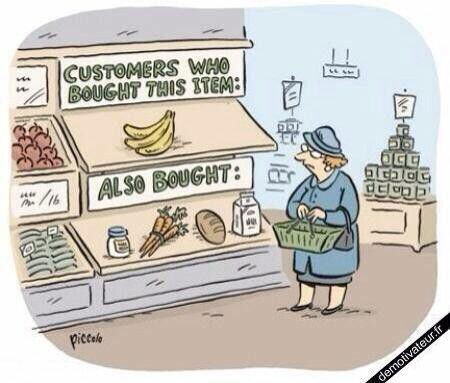
\includegraphics[width=0.5\textwidth]{../figures/recommendation}
    \only<article>{\caption{The recommendation problem}}
    \label{fig:recommendation}
  \end{figure}
  \only<article>{In many machine learning applications, we are dealing with the problem of proposing one or more alternatives to a human. The human can accept zero or more of these choices. As an example, when using an internet search engine, we typically see two things: (a) A list of webpages matching our search terms (b) A smaller list of advertisements that might be relevant to our search. At a high level, }
  \begin{block}{The recommendation problem}
    At time $t$
    \begin{enumerate}
    \item A customer $x_t$ appears. \only<article>{For the internet search problem, $x_t$ would at least involve the search term used.}
    \item We present a choice $a_t$. \only<article>{For the matching website, the choice is ranked list of websites. For the advertisements, however, it is typical }
    \item The customer makes a choice $y_t$. \only<article>{This might include selecting one or more of items suggested in $a_t$.}
    \end{enumerate}
  \end{block}
\end{frame}

\begin{frame}
  
\includegraphics[width=0.5\textwidth]{../figures/netflix}
\end{frame}
\begin{frame}
  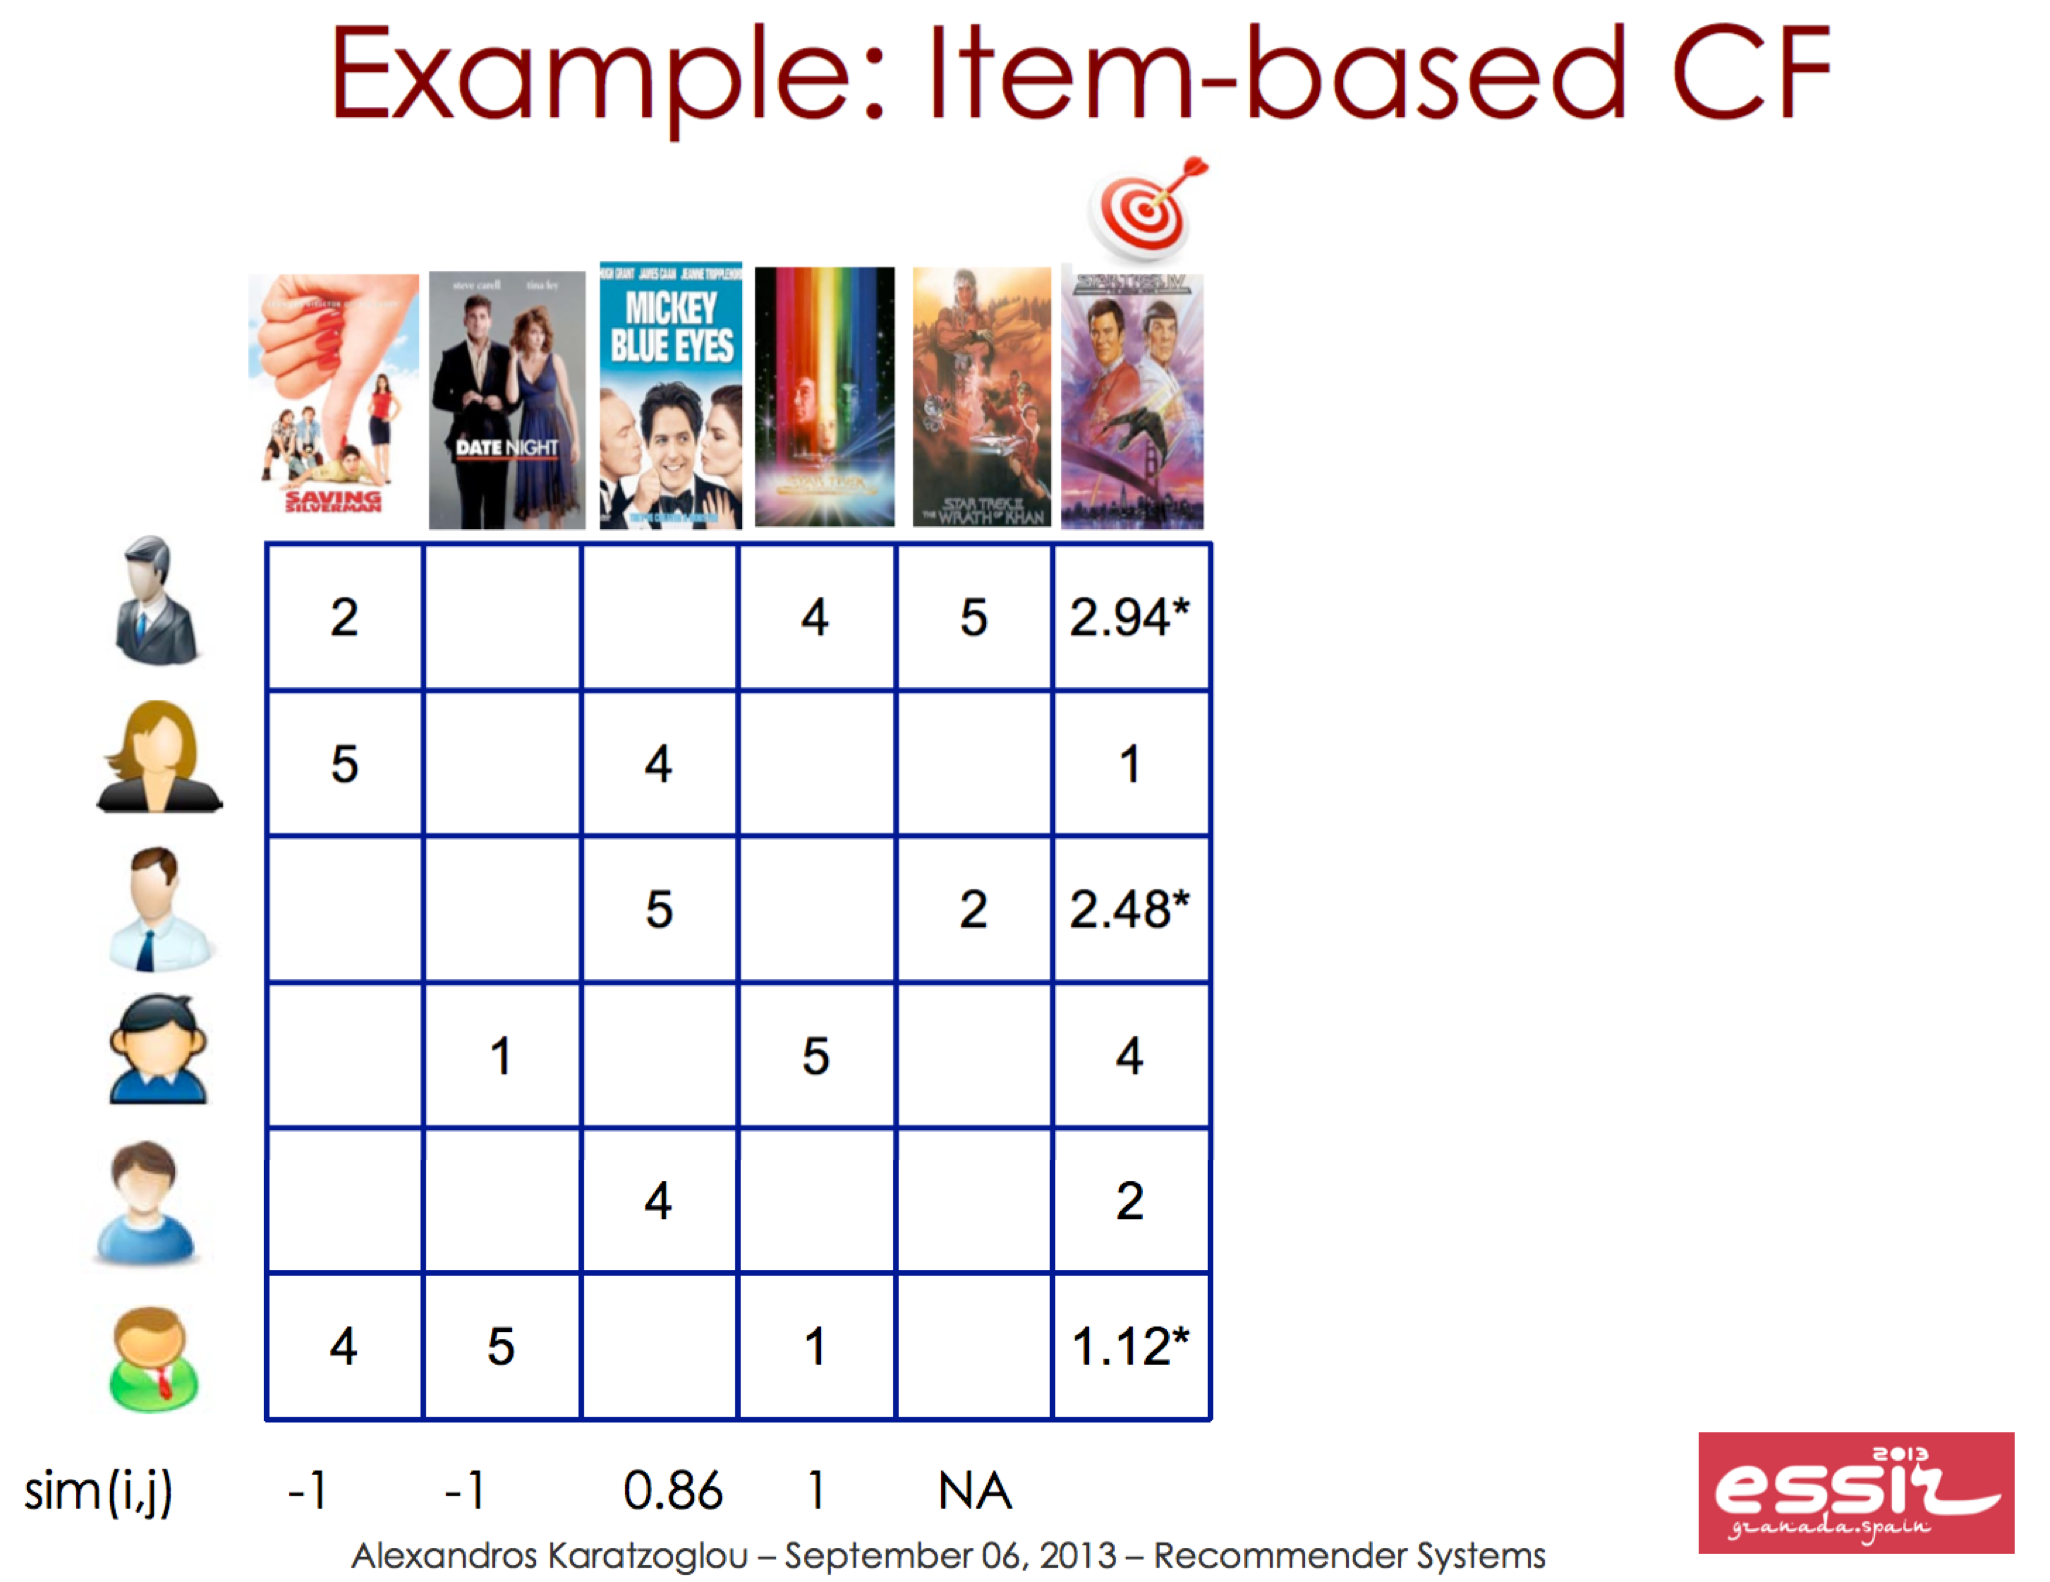
\includegraphics[width=0.9\textwidth]{../figures/recommendationExample-1}
\end{frame}
%%% Local Variables:
%%% mode: latex
%%% TeX-engine: xetex
%%% TeX-master: "notes.tex"
%%% End:
